\documentclass[11pt]{article}
\usepackage[margin=2.5cm]{geometry}
\usepackage{graphicx}
\usepackage{booktabs}
\usepackage{caption}
\usepackage{hyperref}
\usepackage{enumitem}
\usepackage{float}
\usepackage{amsmath,amssymb}
\usepackage[T1]{fontenc}
\usepackage{natbib}
\usepackage{parskip}
\usepackage{authblk}

\setlength{\parskip}{0.5em}
\setlength{\parindent}{0em}

\title{Language Model Comparison, Embedding Ablation, and Downstream Transfer on AG News}

\author[1]{Ng Jun Wei (A0252142U)}
\affil[1]{National University of Singapore}
\date{}

\begin{document}
\maketitle

\begin{abstract}
This report compares four language model families (n-gram, RNN, LSTM, Transformer) trained on AG News under controlled parameter budgets ($\sim$4M parameters each). The Transformer achieves the lowest perplexity (53.6 vs 77.8 LSTM, 96.3 RNN) at modest additional compute cost. An embedding ablation across 9 configurations shows that domain-matched Word2Vec embeddings benefit recurrent models, while the Transformer performs best with trainable scratch embeddings. For downstream 4-class topic classification, frozen Transformer features with a nonlinear head (90.6\%) surpass a bag-of-words baseline (90.2\%), and fine-tuning the Transformer backbone reaches 93.1\% accuracy. Lower language model perplexity correlates with better downstream features, but with diminishing returns for coarse-grained classification.
\end{abstract}

\section{Introduction}

Language models assign probability distributions over token sequences and serve as the foundation for many NLP systems. This report presents a controlled comparison of four language model families on the same English news corpus, followed by an embedding ablation study and a downstream classification evaluation. The goal is to understand how architectural choices and embedding strategies affect both language modeling quality and the usefulness of learned representations for transfer.

All experiments use the \textbf{AG News} dataset, a balanced 4-class topic classification corpus (World, Sports, Business, Sci/Tech) with 96,000 training documents ($\sim$4.7M tokens) and 7,600 test documents. Tokenization is whitespace-based with lowercasing and punctuation separation, retaining the top 20,000 tokens as vocabulary. Sequences are truncated to 128 tokens. For language modeling, the training data is split 80/10/10 into train/val/test; for downstream classification, the original HuggingFace test split (1,900 per class) is used.

To ensure fair comparison, all three neural language models share the same dimensionality (\texttt{embed\_dim} = \texttt{hidden\_dim} = 100), depth (2 layers), regularization (dropout = 0.1), and training regime (Adam, lr = 0.001, gradient clipping at 5.0, batch size 64, 20 epochs). This keeps total parameter counts within 4.06M to 4.28M, so performance differences reflect architectural choices rather than model capacity.

\section{Language Model Training and Comparison}

Five language models are trained on the same data: a bigram and trigram (count-based with Laplace smoothing, $k{=}1$), a 2-layer vanilla RNN with tanh activation, a 2-layer LSTM, and a 2-layer decoder-only Transformer (GPT-style, 4 attention heads, $d_{ff}{=}400$, learned positional embeddings with causal masking).

\begin{table}[H]
\centering\small
\begin{tabular}{llr}
\toprule
\textbf{Model} & \textbf{Architecture} & \textbf{Parameters} \\
\midrule
Bigram & Count-based, Laplace smoothing & N/A \\
Trigram & Count-based, Laplace smoothing & N/A \\
RNN & 2-layer vanilla RNN, tanh & 4,060,400 \\
LSTM & 2-layer LSTM & 4,181,600 \\
Transformer & 2-layer decoder-only, 4 heads, $d_{ff}{=}400$ & 4,275,600 \\
\bottomrule
\end{tabular}
\caption{Model architectures and parameter counts.}
\label{tab:models}
\end{table}

\subsection{Results}

\begin{table}[H]
\centering\small
\begin{tabular}{lrrrr}
\toprule
\textbf{Model} & \textbf{Val PPL} & \textbf{Test PPL} & \textbf{Train Time} & \textbf{Inference (ms/batch)} \\
\midrule
Bigram & 860.44 & 849.76 & 5.3s & 4.73 \\
Trigram & 3791.59 & 3735.70 & 10.0s & 6.03 \\
RNN & 97.46 & 96.26 & 1878.5s ($\sim$94s/ep) & 0.90 \\
LSTM & 78.75 & 77.82 & 1997.8s ($\sim$100s/ep) & 0.94 \\
Transformer & \textbf{54.07} & \textbf{53.59} & 2101.9s ($\sim$105s/ep) & 2.26 \\
\bottomrule
\end{tabular}
\caption{Perplexity, training time, and inference speed across all language models.}
\label{tab:ppl}
\end{table}

\begin{figure}[H]
\centering
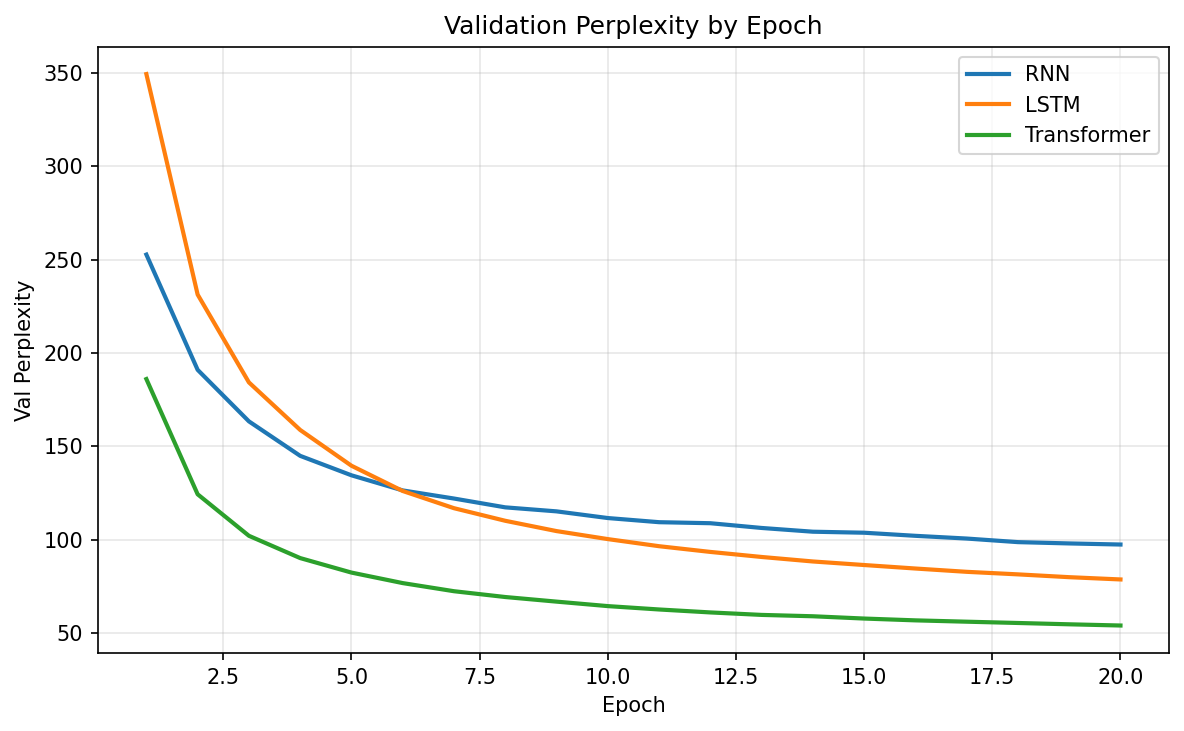
\includegraphics[width=0.62\textwidth]{../outputs/plots/part1_val_perplexity.png}
\caption{Validation perplexity by epoch. The Transformer converges fastest and reaches the lowest perplexity. All three neural models continue improving at epoch 20, with no sign of overfitting (Figure~\ref{fig:overfit}).}
\label{fig:valppl}
\end{figure}

\begin{figure}[H]
\centering
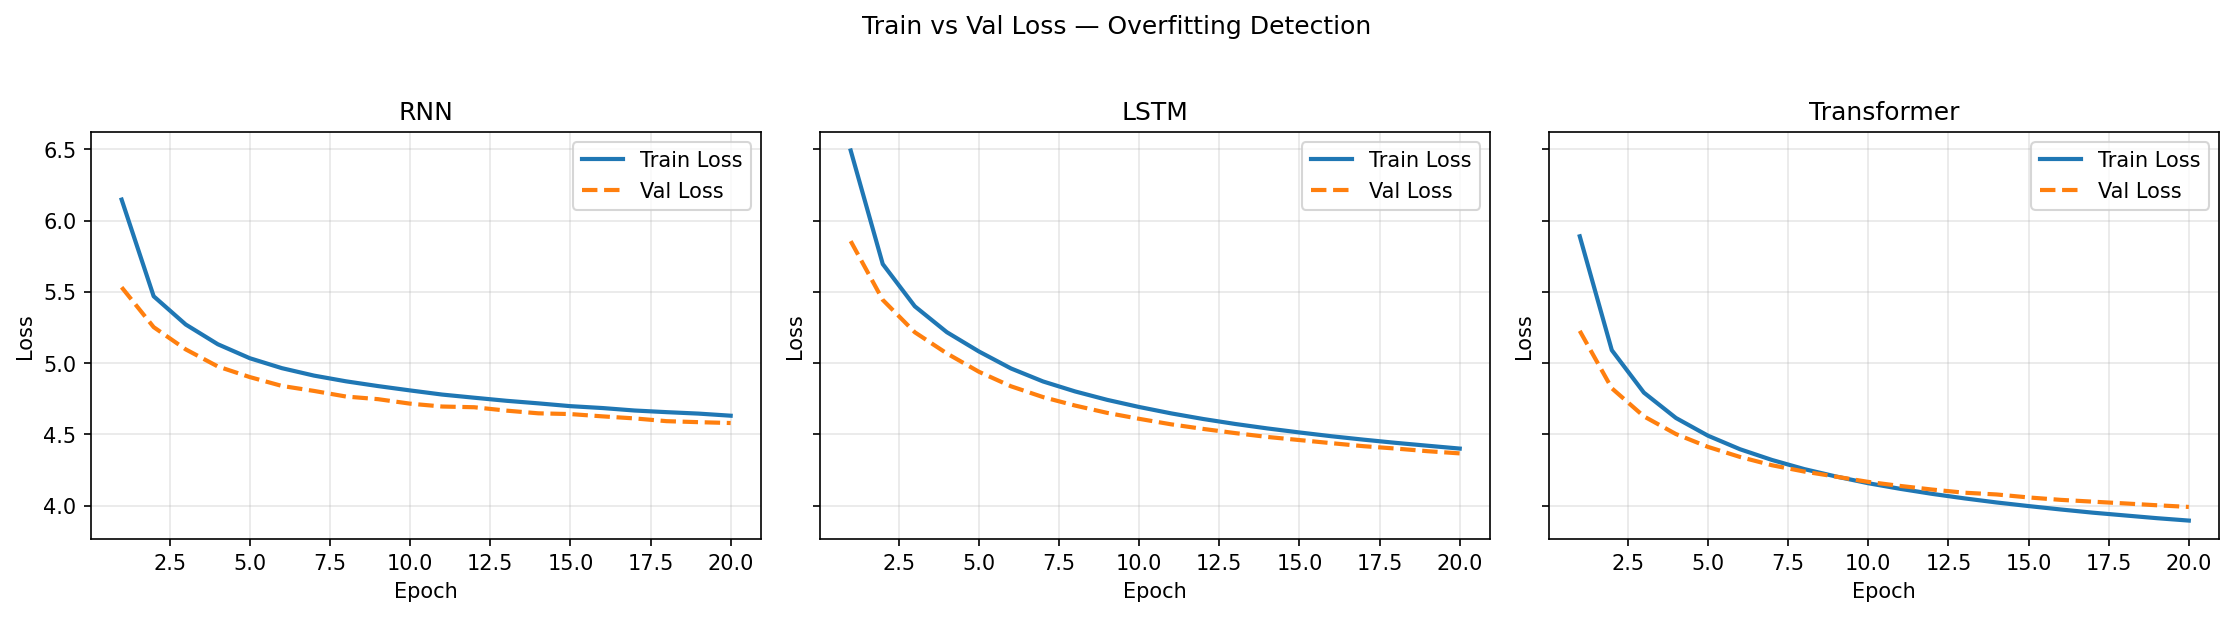
\includegraphics[width=0.92\textwidth]{../outputs/plots/part1_overfitting.png}
\caption{Train vs validation loss. The train-val gap remains small throughout, confirming that 20 epochs is appropriate for this dataset size.}
\label{fig:overfit}
\end{figure}

\subsection{Analysis}

The n-gram models serve as a useful baseline but have far higher perplexity. The trigram (PPL 3736) performs \emph{worse} than the bigram (PPL 850) because Laplace smoothing distributes mass uniformly across unseen events, and with 1.0M distinct trigram histories (vs 60K bigram), sparsity is far more severe.

Among neural models, the hierarchy is clear: Transformer (PPL 53.6) $>$ LSTM (PPL 77.8) $>$ RNN (PPL 96.3). The LSTM's 19\% improvement over the RNN comes from its gating mechanism, which provides a gradient highway through the cell state. The Transformer extends this further: self-attention creates direct connections between any two positions, avoiding the sequential bottleneck entirely. Its PPL is 31\% lower than the LSTM's.

This quality comes at a cost: the Transformer is the slowest model in training (105s/epoch vs 100s for LSTM, 94s for RNN) and inference (2.26~ms/batch vs $\sim$0.9~ms), reflecting $O(n^2)$ attention overhead at this small scale.

In generated text, n-gram samples lose topic consistency within a few words. The RNN drifts after $\sim$15 tokens, the LSTM holds slightly longer, and the Transformer produces the most topically coherent passages.

\section{Embedding Variants and Ablation}

To understand how the embedding layer affects language modeling, the default trainable embeddings are replaced with two frozen alternatives and each neural model is retrained. This gives a $3 \times 3$ grid of 9 experiments:

\begin{itemize}[nosep]
\item \textbf{Scratch}: standard trainable embeddings (nn.Embedding, 100-dim), randomly initialized.
\item \textbf{W2V frozen}: Word2Vec (Skip-gram, dim=100, window=5) trained on the AG News \emph{training set only} via Gensim, then frozen. Coverage: 99.98\% (19,996/20,000).
\item \textbf{GloVe pretrained frozen}: \texttt{glove-wiki-gigaword-100}, a public embedding from Wikipedia + Gigaword. Coverage: 98.8\% (19,768/20,000).
\end{itemize}
Freezing the embedding removes $\sim$2M parameters from gradient updates, so frozen variants have roughly half the trainable parameters of scratch.

\subsection{Results}

\begin{table}[H]
\centering\small
\begin{tabular}{lcccc}
\toprule
\textbf{Model} & \textbf{Params (scratch/frozen)} & \textbf{Scratch PPL} & \textbf{W2V PPL} & \textbf{GloVe PPL} \\
\midrule
RNN & 4.06M / 2.06M & 96.26 & \textbf{93.13} & 111.39 \\
LSTM & 4.18M / 2.18M & 78.00 & \textbf{75.06} & 83.12 \\
Transformer & 4.28M / 2.28M & \textbf{53.83} & 57.65 & 60.76 \\
\bottomrule
\end{tabular}
\caption{Test perplexity by embedding variant. Bold = best per model.}
\label{tab:embed}
\end{table}

\begin{figure}[H]
\centering
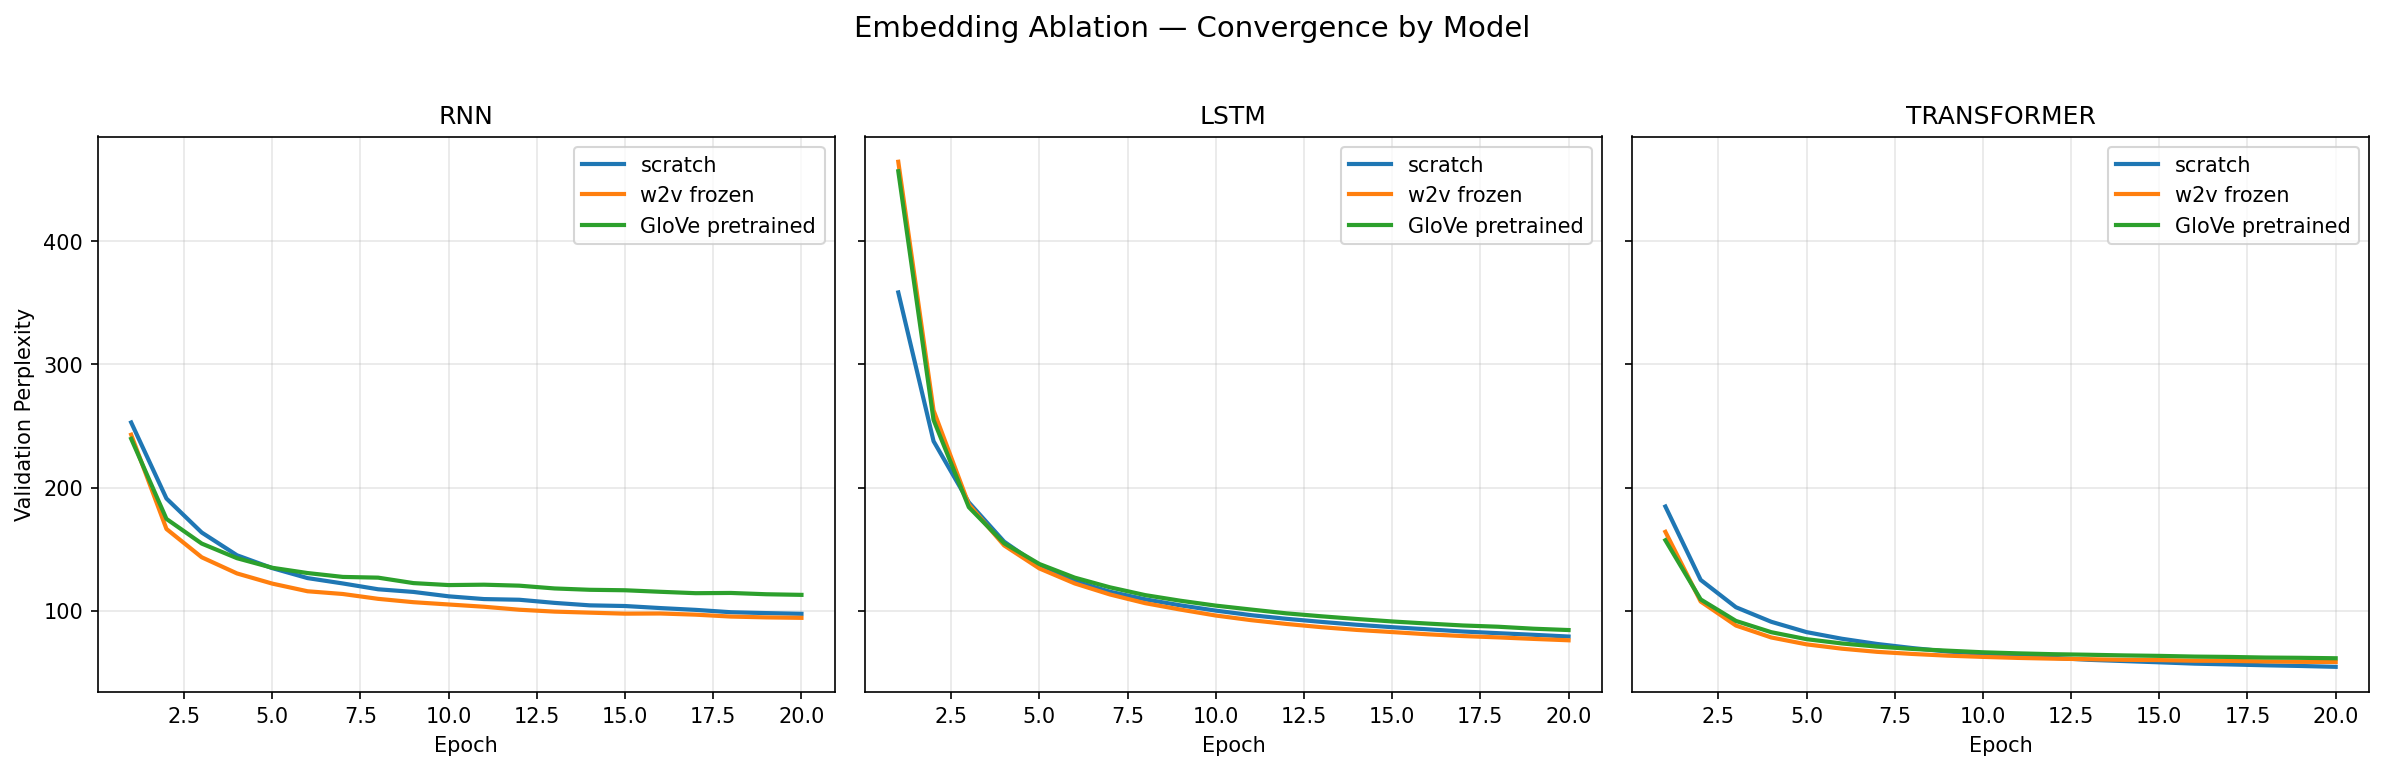
\includegraphics[width=\textwidth]{../outputs/plots/part2_convergence.png}
\caption{Validation perplexity over 20 epochs for each model-embedding combination.}
\label{fig:convergence}
\end{figure}

\begin{figure}[H]
\centering
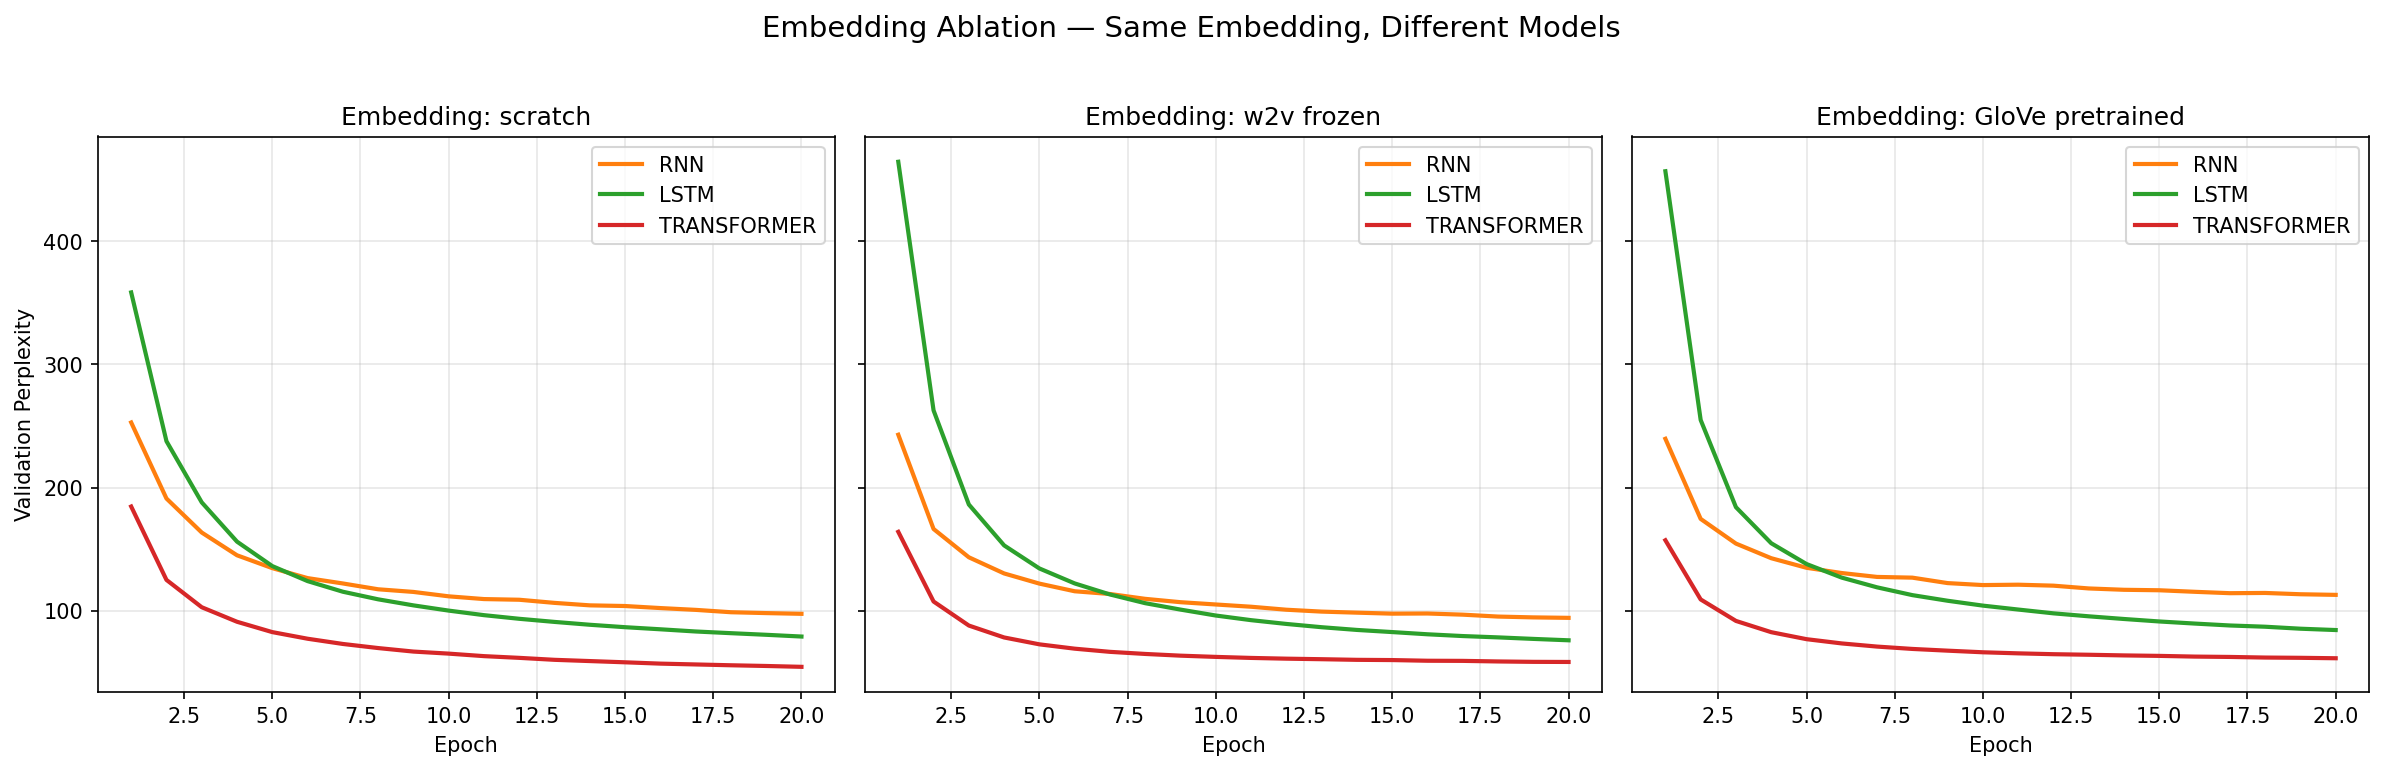
\includegraphics[width=\textwidth]{../outputs/plots/part2_cross_model.png}
\caption{Holding the embedding constant, the Transformer consistently outperforms LSTM and RNN.}
\label{fig:crossmodel}
\end{figure}

\subsection{Convergence Speed}

\begin{table}[H]
\centering\small
\begin{tabular}{lccc}
\toprule
\textbf{Run} & \textbf{Epoch-1 PPL} & \textbf{Best PPL} & \textbf{Gap} \\
\midrule
RNN scratch & 252.80 & 97.46 & 155.34 \\
RNN W2V & 242.86 & 94.18 & 148.68 \\
RNN GloVe & 239.55 & 112.84 & 126.71 \\
LSTM scratch & 358.39 & 79.01 & 279.38 \\
LSTM W2V & 464.46 & 75.96 & 388.51 \\
LSTM GloVe & 456.77 & 84.28 & 372.49 \\
TF scratch & 184.57 & 54.42 & 130.16 \\
TF W2V & 164.01 & 58.37 & 105.65 \\
TF GloVe & 157.18 & 61.39 & 95.79 \\
\bottomrule
\end{tabular}
\caption{Epoch-1 perplexity as a convergence speed signal.}
\label{tab:convergence}
\end{table}

\subsection{Analysis}

\textbf{W2V dominates for recurrent models.} W2V frozen achieves the best test perplexity for both RNN (93.1 vs 96.3 scratch) and LSTM (75.1 vs 78.0). W2V was self-trained on AG News, so it encodes domain-specific co-occurrence patterns with near-perfect coverage. GloVe, despite a much larger training corpus (Wikipedia + Gigaword), encodes general-purpose semantics that are less aligned with news text.

\textbf{Scratch wins for Transformer.} Self-attention reshapes representations at every layer, effectively learning task-optimal embeddings during training. With 2M additional trainable embedding parameters, the scratch Transformer has more capacity to specialize. Recurrent models, processing tokens through a fixed-size hidden state, benefit more from good initialization.

\textbf{LSTM convergence anomaly.} LSTM scratch (epoch-1 PPL 358) starts \emph{better} than frozen variants (W2V 464, GloVe 457), the opposite of RNN and Transformer. LSTM gate initialization is calibrated for random-scale inputs; pretrained embeddings with a different scale cause suboptimal initial gate behavior. Despite the slow start, W2V LSTM still converges to the best final perplexity.

\textbf{GloVe is worst everywhere.} Domain mismatch (general vs.\ news) and lower coverage (98.8\% vs 99.98\%) outweigh the benefit of larger pretraining data.

\section{Downstream Task with Learned Representations}

Having trained language models of varying quality, the central question is: do better language models produce better features for classification? Frozen representations are extracted from each trained LM and used for AG News topic classification.

\subsection{Feature Extraction and Methods}

For each LM, a forward pass is run over every document to extract hidden states at the final layer, \textbf{mean-pooled} across non-padding positions to produce a 100-dimensional feature vector per document.

\begin{table}[H]
\centering\small
\begin{tabular}{ll}
\toprule
\textbf{Method} & \textbf{Description} \\
\midrule
BoW + LogReg & CountVectorizer + logistic regression (sklearn) \\
Frozen LM + Linear & Frozen features $\rightarrow$ linear layer (100$\rightarrow$4) \\
Frozen LM + MLP & Frozen features $\rightarrow$ 1-hidden-layer MLP (100$\rightarrow$128$\rightarrow$4, ReLU) \\
Fine-tuned TF + Linear & End-to-end fine-tuning, differential LR (LM: 1e-4, head: 1e-3) \\
\bottomrule
\end{tabular}
\caption{Downstream classification methods.}
\label{tab:methods}
\end{table}

Frozen probes are applied to all three backbones; only the Transformer is fine-tuned as the strongest backbone. All classifiers train for 10 epochs with Adam.

\subsection{Results}

\begin{table}[H]
\centering\small
\begin{tabular}{lcccccc}
\toprule
\textbf{Method} & \textbf{Acc} & \textbf{F1} & \textbf{World} & \textbf{Sports} & \textbf{Business} & \textbf{Sci/Tech} \\
\midrule
BoW + LogReg & 0.902 & 0.902 & 0.906 & 0.961 & 0.865 & 0.877 \\
RNN frozen + Linear & 0.840 & 0.840 & 0.845 & 0.920 & 0.794 & 0.801 \\
RNN frozen + MLP & 0.857 & 0.857 & 0.867 & 0.930 & 0.812 & 0.818 \\
LSTM frozen + Linear & 0.871 & 0.871 & 0.873 & 0.945 & 0.824 & 0.844 \\
LSTM frozen + MLP & 0.883 & 0.883 & 0.882 & 0.948 & 0.842 & 0.859 \\
TF frozen + Linear & 0.880 & 0.879 & 0.886 & 0.947 & 0.839 & 0.846 \\
TF frozen + MLP & 0.906 & 0.906 & 0.915 & 0.963 & 0.869 & 0.876 \\
\textbf{TF fine-tuned + Linear} & \textbf{0.931} & \textbf{0.931} & \textbf{0.939} & \textbf{0.978} & \textbf{0.901} & \textbf{0.904} \\
\bottomrule
\end{tabular}
\caption{Downstream classification results. Per-class columns show F1 scores.}
\label{tab:downstream}
\end{table}

\begin{figure}[H]
\centering
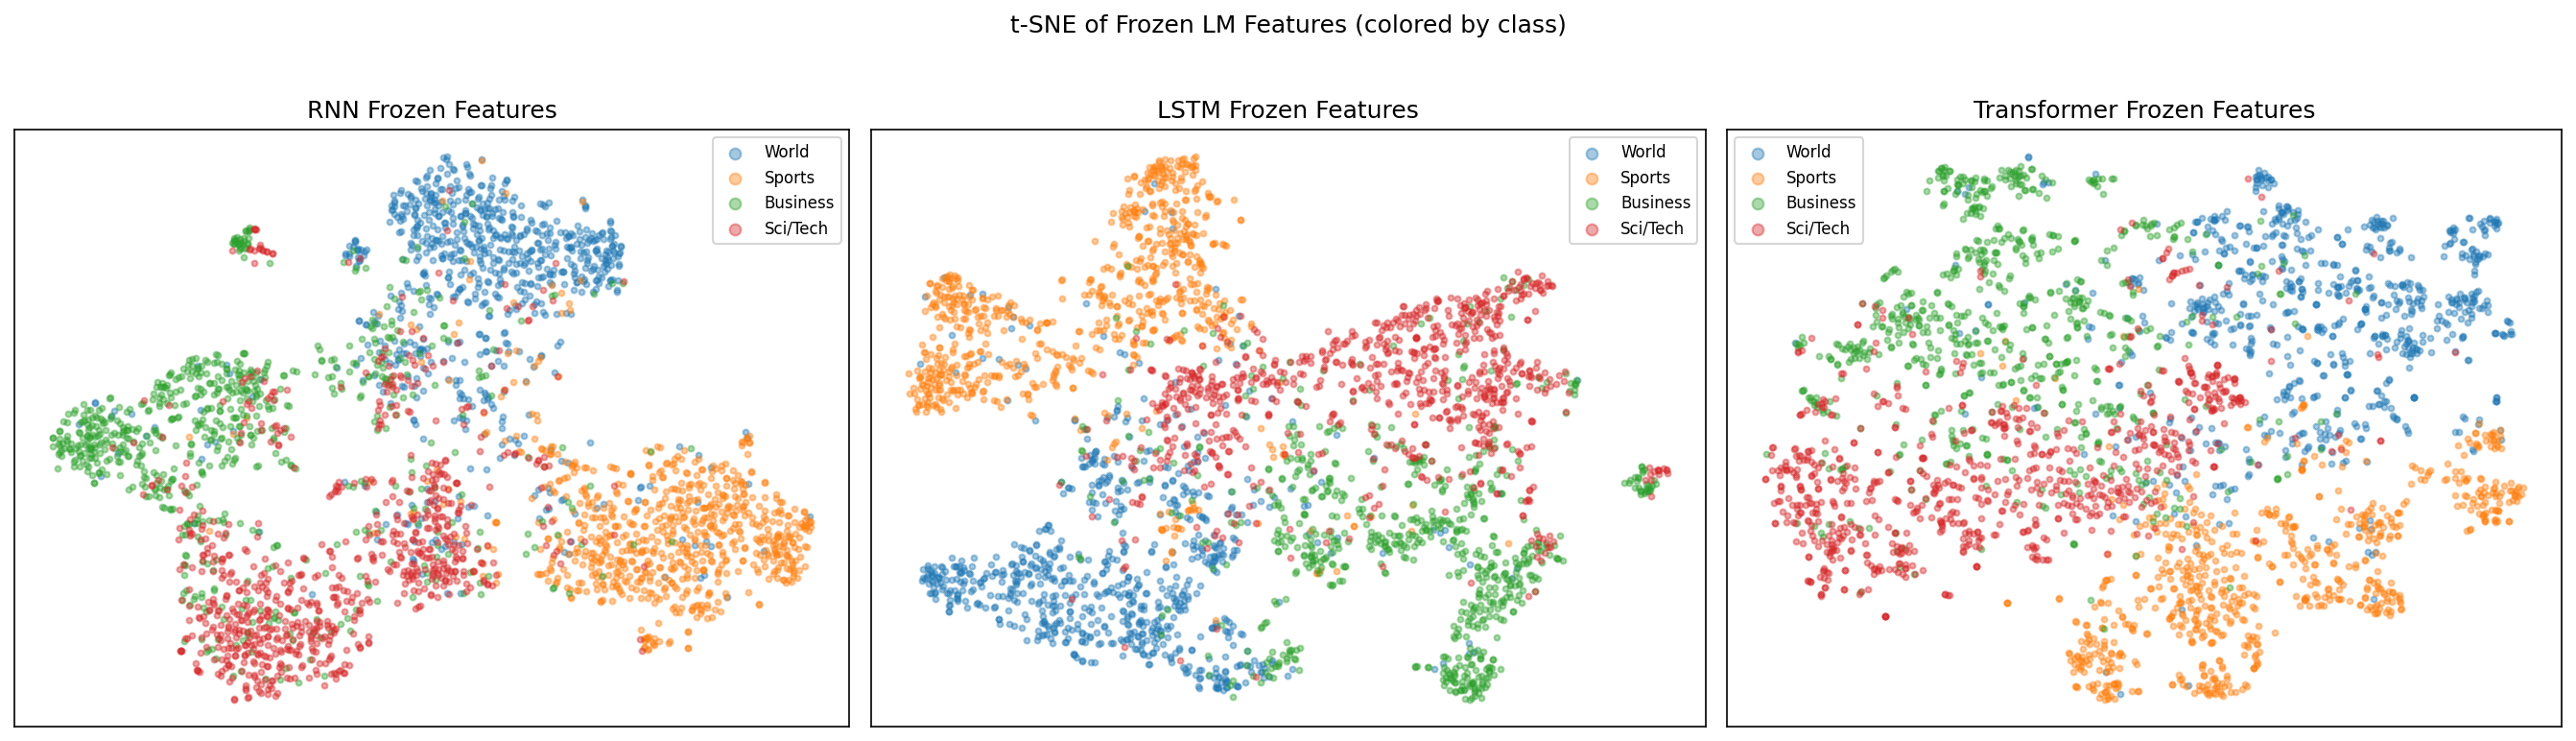
\includegraphics[width=\textwidth]{../outputs/plots/part3_tsne.png}
\caption{t-SNE of frozen LM features (3,000 test samples). Transformer features show the clearest cluster separation; RNN features are the most diffuse.}
\label{fig:tsne}
\end{figure}

\begin{figure}[H]
\centering
\begin{minipage}{0.48\textwidth}
\centering
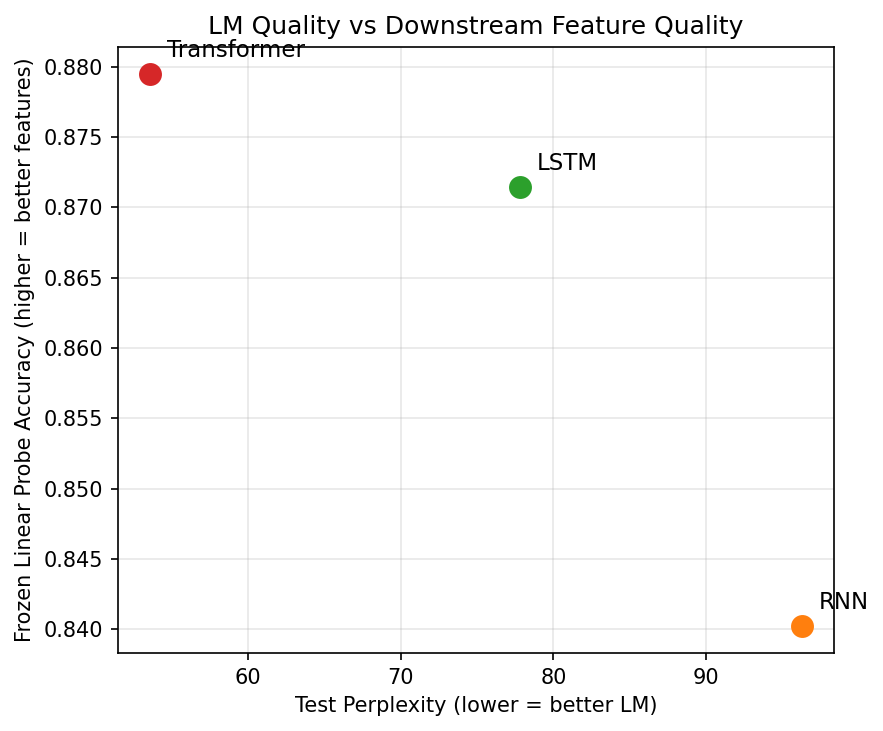
\includegraphics[width=\textwidth]{../outputs/plots/part3_ppl_vs_accuracy.png}
\caption{Perplexity vs frozen linear probe accuracy. Better LMs produce better features, with diminishing returns.}
\label{fig:pplvsacc}
\end{minipage}\hfill
\begin{minipage}{0.48\textwidth}
\centering
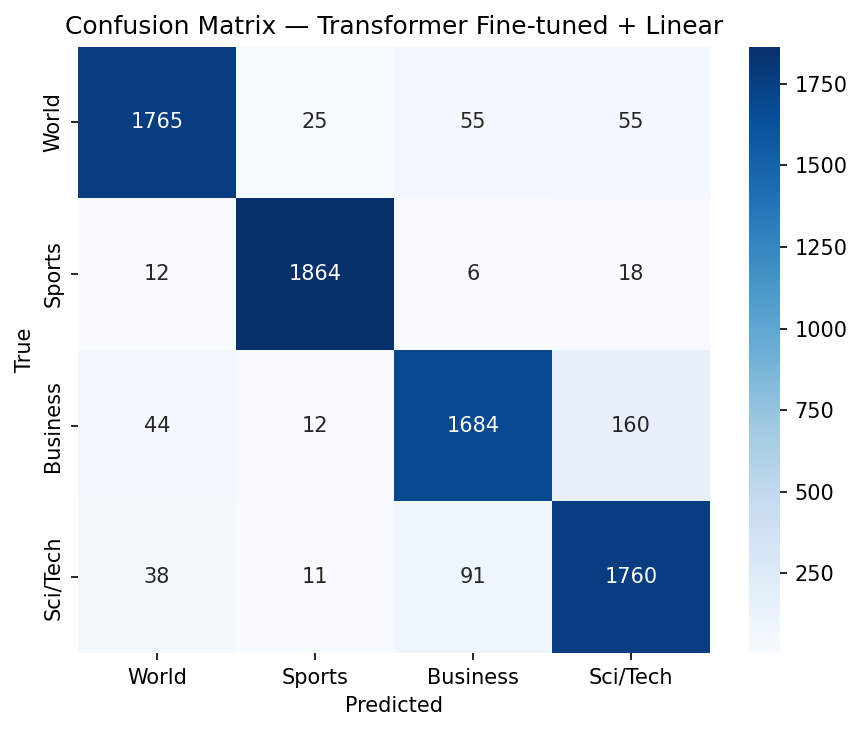
\includegraphics[width=\textwidth]{../outputs/plots/part3_confusion_matrix.png}
\caption{Confusion matrix for the fine-tuned Transformer (best model).}
\label{fig:confmat}
\end{minipage}
\end{figure}

\begin{figure}[H]
\centering
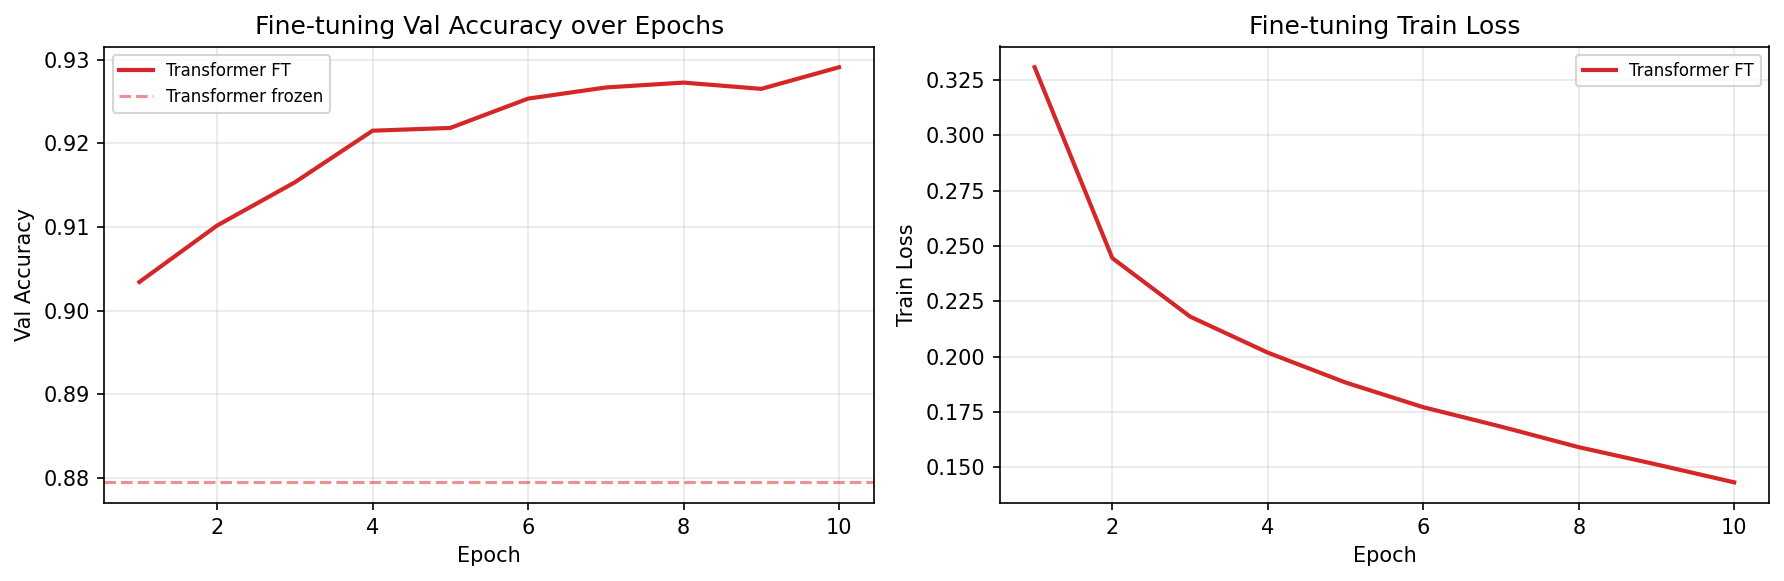
\includegraphics[width=0.82\textwidth]{../outputs/plots/part3_finetune_dynamics.png}
\caption{Fine-tuning dynamics. Val accuracy rises from 90.1\% to 92.8\% over 10 epochs with no overfitting.}
\label{fig:finetune}
\end{figure}

\subsection{Analysis}

\textbf{BoW outperforms all frozen linear probes.} A simple bag-of-words (90.2\%) beats every frozen LM + linear head, including the Transformer (88.0\%). Topic classification depends on \emph{which words appear}, and BoW captures this directly. Frozen LM features, shaped by next-token prediction, do not explicitly encode class-discriminative information.

\textbf{Nonlinear heads unlock the Transformer.} MLP gains are uneven: RNN +1.7\%, LSTM +1.2\%, Transformer +2.6\%. The larger gain indicates Transformer features encode richer nonlinear structure from self-attention. TF frozen + MLP (90.6\%) is the only frozen config surpassing BoW.

\textbf{PPL correlates with feature quality, with diminishing returns.} RNN (PPL 96.3, Acc 84.0\%) $\rightarrow$ LSTM (PPL 77.8, Acc 87.1\%) $\rightarrow$ Transformer (PPL 53.6, Acc 88.0\%). The 31\% PPL drop LSTM$\rightarrow$TF yields only +0.9\% linear probe accuracy, as further perplexity gains capture patterns that do not directly help coarse topic classification.

\textbf{Fine-tuning gives the largest gain.} The fine-tuned Transformer (93.1\%) gains +5.1\% over frozen + linear and +2.5\% over frozen + MLP. Fine-tuning reshapes representations from ``what word comes next'' to ``what topic is this.'' Val accuracy climbs from 90.3\% to 92.9\% over 10 epochs with no overfitting.

\textbf{Per-class patterns.} Sports is easiest (F1 0.92--0.98); Business is hardest (F1 0.79--0.90). Fine-tuning helps weak classes most: Business F1 improves from 0.84 to 0.90 (+6\% absolute).

\textbf{Connection to LM architecture.} More expressive architectures produce richer representations, but that richness is only accessible through nonlinear probes or fine-tuning. Recurrent models compress through a fixed-size hidden state, yielding more linearly separable features. The Transformer distributes information across a higher-dimensional attention-derived space that requires more downstream capacity to exploit, but achieves the best results when given that capacity.

\section{Experimental Controls}

\begin{itemize}[nosep]
\item \textbf{Parameter fairness:} All neural LMs have 4.06--4.28M parameters. The shared embedding (20K $\times$ 100 = 2M) and output projection (100 $\times$ 20K = 2M) dominate; differences come only from model cores.
\item \textbf{Same pipeline:} Same tokenizer, vocabulary, splits, and max sequence length (128).
\item \textbf{No data leakage:} W2V trained only on the training split. Zero split overlap verified.
\item \textbf{Sanity checks:} All models overfit one batch ($>$50\% loss drop); all parameters receive gradients; Transformer causal mask verified.
\item \textbf{Hardware:} All experiments run on a single NVIDIA GeForce RTX 4060 GPU.
\item \textbf{Reproducibility:} Seed 42. Hyperparameters centralized in \texttt{configs/default.yaml}.
\end{itemize}

\section{Limitations}

\begin{itemize}[nosep]
\item \textbf{Tokenization:} Only whitespace splitting with lowercasing is used, with no subword tokenization (BPE/WordPiece). This inflates the vocabulary with rare surface forms and limits generalization across morphological variants.
\item \textbf{Training not converged:} All neural models are still improving at epoch 20 with no plateau reached. Longer training or a learning rate schedule would likely improve all models, though relative rankings are unlikely to change.
\item \textbf{Single dataset:} All results are specific to AG News (short news snippets, 4-class topic classification). Findings about embedding choices and downstream transfer may not generalize to longer documents, more fine-grained tasks, or other domains.
\item \textbf{Small scale:} Models are 2-layer, 100-dim ($\sim$4M parameters). At larger scales, the Transformer's advantage over recurrent models would likely widen due to better parallelism and deeper attention stacking.
\item \textbf{Frozen-only embeddings:} The ablation compares frozen pretrained vs.\ trainable scratch, but does not test \emph{fine-tuned} pretrained embeddings (initialize from W2V/GloVe then allow gradient updates), which could combine the benefits of both approaches.
\end{itemize}

\section{Conclusion}

Across all three parts of this study, the Transformer consistently outperforms recurrent and n-gram models in language modeling quality, produces the richest downstream features, and benefits most from fine-tuning. Domain-matched Word2Vec embeddings help recurrent models but not the Transformer, which learns better embeddings from scratch. The relationship between language model perplexity and downstream classification accuracy is positive but sublinear, suggesting that beyond a quality threshold, further LM improvements capture linguistic structure that does not directly benefit coarse-grained topic classification. These findings highlight the importance of matching both the model architecture and the embedding strategy to the target task and domain.

\end{document}
